\section{系统误差分析}
这一节我们讨论分析方法和工具可能带来的系统误差和误差的估计方法。
根据$\mathcal{B}$的计算公式,产额$N$和效率$\epsilon$的不确定性都会影响$\mathcal{B}$的测量。
所有可能的误差来源应该都是通过$N$或$\epsilon$影响到最终的结果。
所以可以将误差来源视为两大类:一类来自重建过程,它是$\epsilon$的误差的来源;另一类来自拟合(或其他确定产额的方法),它是$N$的误差的来源。
当然,也要视具体情况由测量公式来定,有时候也会有外部输入的系统误差。
一般地,效率的误差是指在事例筛选过程中对效率损失的估计的偏差。
具体可能包括:对触发效率、寻迹效率、PID(粒子鉴别)效率、光子重建效率、$\pi^{0}$/$\eta$/$K_{S}^{0}$等中间态粒子的重建效率、
其他约束某物理量在信号窗带来的效率、运动学拟合带来的效率偏差,以及MC产生子的模型对真实过程的模拟不完全正确等方面。
对于$N$的估计的偏差,一般是确定信号数的方法带来的系统偏差。可能的来源有:拟合方法(拟合用到的形状,范围)、本底估计(峰本底扣除,边带区减除)等。
对于系统误差估计要具体情况具体分析,一般要看这一原因会影响什么?只影响产额$N$还是只影响效率$\epsilon$还是既影响产额$N$又影响效率$\epsilon$;
常见的分析方法一般有这么几种:用MC数据之间的差异来估计、变化该项因素看影响量的变化、控制样本研究等方法。


具体到我们这个分析,通过计算公式我们可以看出,单标记侧的系统误差可以认为已经被约掉了,我们只需要考虑双标记一侧的系统误差就可以了。
需要考虑的系统误差有$K$介子的寻迹效率、PID(粒子鉴别)效率、单标计测可能的小量峰状本底、双标记侧$M_{\rm miss}$谱的拟合、$M_{\rm BC}$要求、MC有限的统计量和MC产生子的模型对真实过程的模拟不完全正确。
我们先将其列在表~\ref{tab:sys_err}中,然后再逐条解释。

\begin{table}[hp]
  \begin{center}
  %\footnotesize
    \caption{系统误差总结表,以百分比的形式展示。}
  \begin{tabular}{l|c|c}
      \hline \hline
			误差来源            &  $\LtoXiK(\%)$ &  $\LtoXisK(\%)$ \\
			\hline  
			 MC模型          &    3.2     &     3.9     \\
			$K$介子寻迹效率  &    1.0      &    1.0      \\
			$K$介子粒子鉴别   &    1.0      &    1.0      \\
			$M_{\rm miss}$拟合&    5.2     &     3.7     \\
单标记侧峰状本底   &    0.8     &     0.8     \\
			$M_{\rm BC}$要求      &    2.2     &     2.4    \\
      MC 统计量     & $\cdots$   &   $\cdots$    \\
			\hline
      Total             &    6.7      &    6.1     \\
      \hline\hline
    \end{tabular}
    \label{tab:sys_err}
  \end{center}
  \end{table}
%%%%%%%%%%%%%%%%%%%%%%%%%%%%%%%%%%%%%

\subsection{寻迹和粒子鉴别}
在我们的信号衰变过程$\LtoXiXisK$中,$K^{+}$的动量分布如图~\ref{fig:pKaon_data}所示,分布在0.3$\gevc$到0.8$\gevc$之间。
对于寻迹和粒子鉴别带来的系统误差设为1\%是安全且合理的。

\begin{figure*}[hp]
\centering
\subfigure[]
{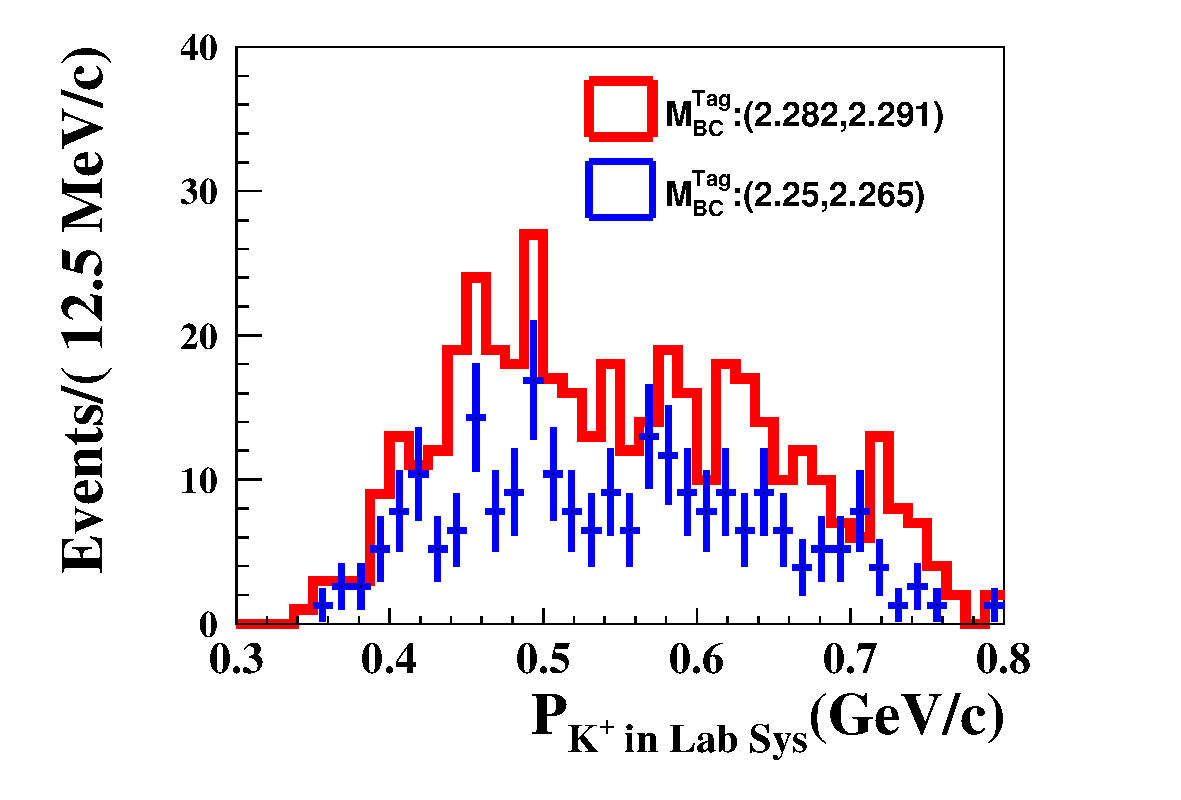
\includegraphics[width=0.45\textwidth]{chap2_P_KinLab_data} }
\hspace{1pt}
\subfigure[]
{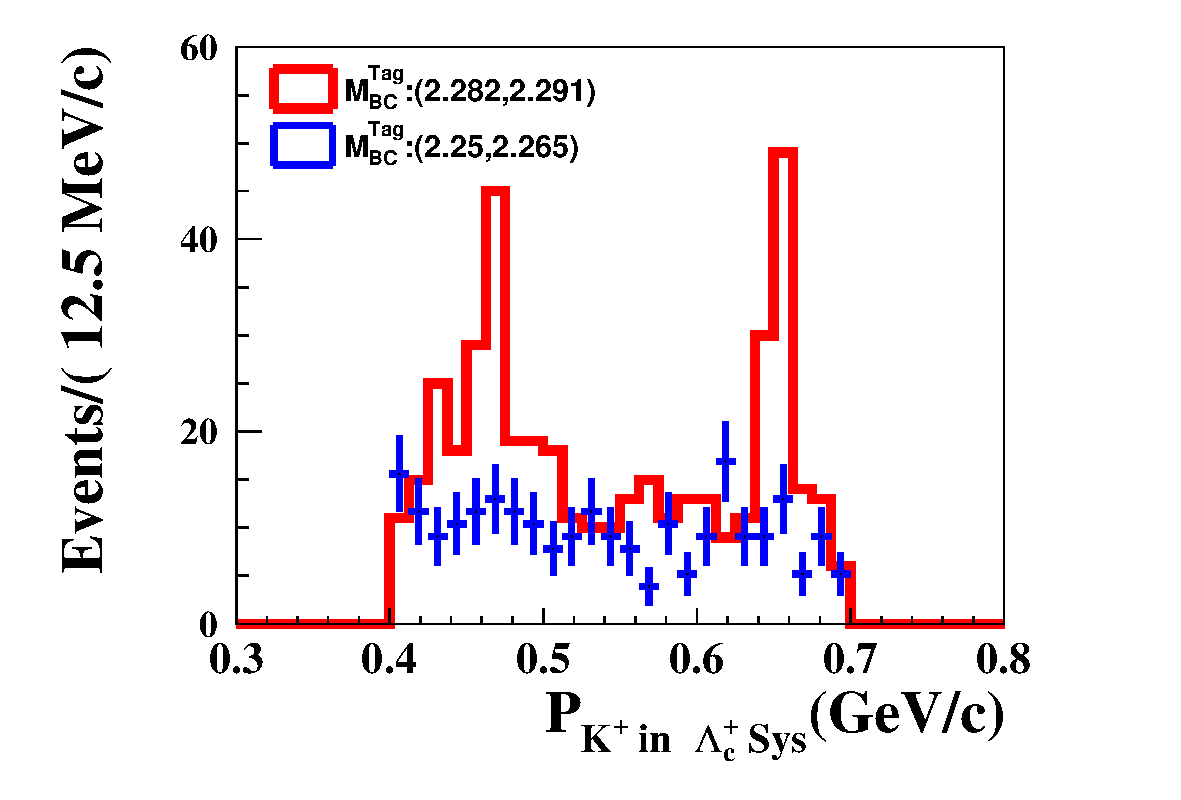
\includegraphics[width=0.45\textwidth]{chap2_P_KinLc_data}}
\hspace{1pt}
\subfigure[]
{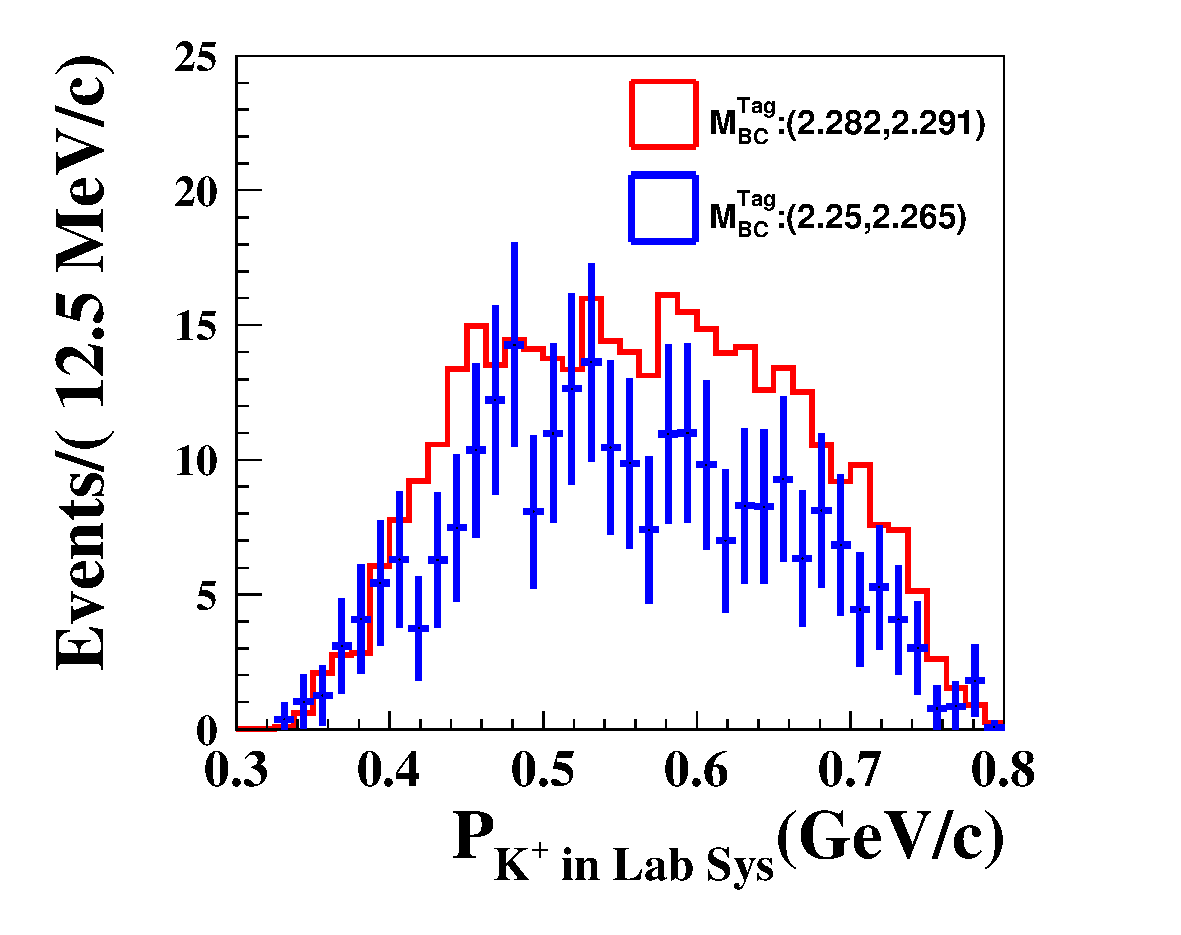
\includegraphics[width=0.45\textwidth]{chap2_P_KinLab_mc}}
\hspace{1pt}
\subfigure[]
{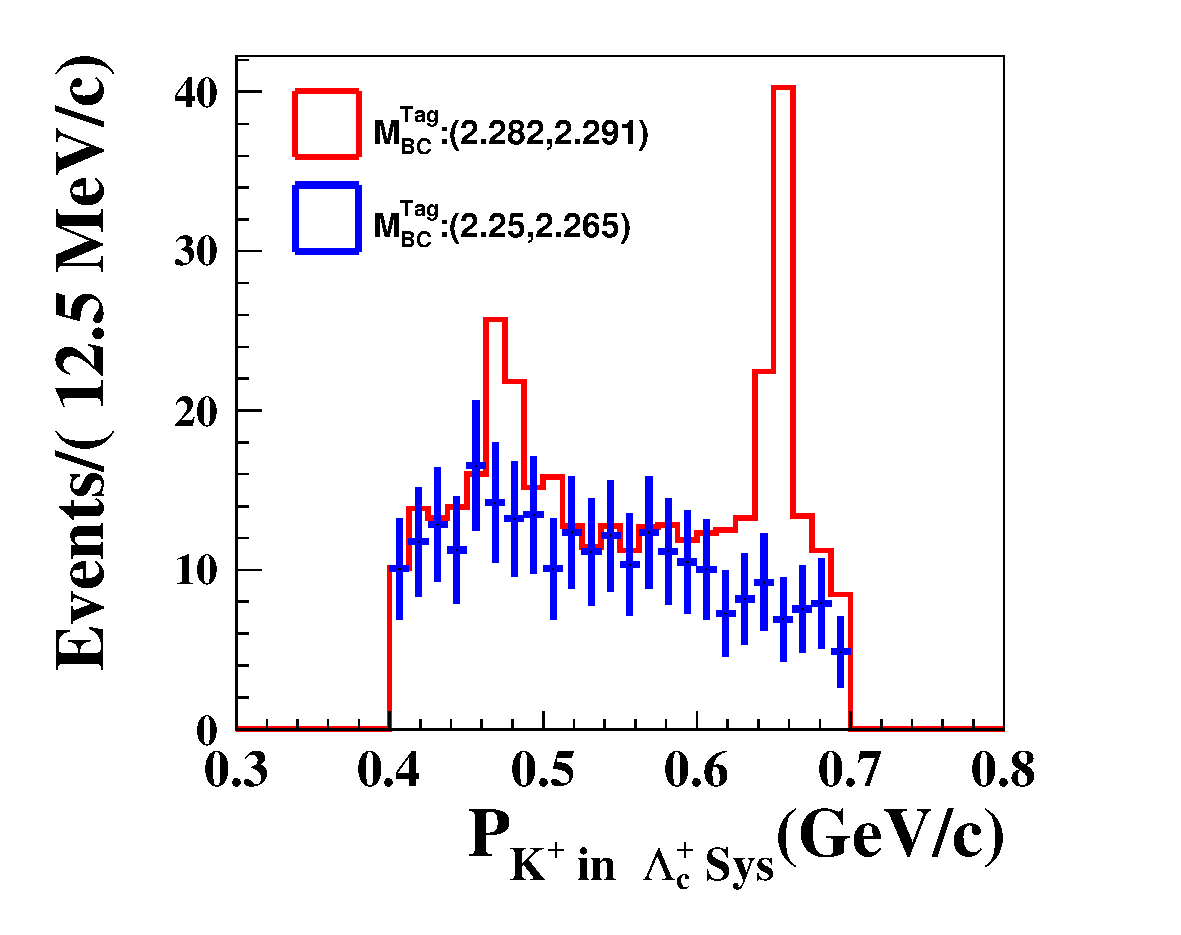
\includegraphics[width=0.45\textwidth]{chap2_P_KinLc_mc}}
\caption{\textbf{数据}[Fig.(a) 和 (b)]中和 \textbf{Cocktail MC}[Fig.(c) 和 (d)]中$K^{+}$介子的动量分布。}
\label{fig:pKaon_data}
\end{figure*}

\subsection{$M_{\rm miss}$拟合}

我们通过调整$M_{\rm miss}$谱的拟合范围和本底形状来估计由于拟合带来的系统误差。
拟合范围我们从(1.1,1.65)$\gevcc$改变到(1.2,1.65)$\gevcc$,发现不会对$\XiXisK$的产额产生影响。
另外,中心结果里面我们采用二阶多项式来描述本底。为了估计本底形状的选择带来的系统误差,我们采用一阶多项式来拟合,得到信号数目的相对变化作为由拟合带来的系统误差。


\subsection{有限的MC模拟统计量}
MC模拟的量的统计误差作为效率的系统误差。我们模拟了大量的MC样本,此项误差可以忽略。

\subsubsection{单标记侧峰状本底。}
虽然我们目测单标记侧$M_{\rm BC}$谱上基本没有峰状本底的贡献,
但是为了保险起见我们还是对本底MC,假设有信号进行了拟合。
如果将这部分效应考虑到数据的统计量下,会贡献0.8\%的系统误差。

\subsection{$M_{\rm BC}$窗口要求} 
MC与数据之间的分辨差异用来修正MC中$M_{\rm BC}$的分布。
如果我们不做修正的话,由$M_{\rm BC}$窗口要求带来的系统误差对$\LtoXiK$和$\LtoXisK$分别为2.2$\%$和2.4$\%$.

\subsection{信号模型}
众所周知,MC模拟与数据之间的一致性好坏直接影响着MC估计效率的准确性。
对于$\LtoXiK$和$\LtoXisK$,$K^+$介子的空间极角分布模拟的好坏是我们要考虑的一项影响双标记效率的系统误差。
我们用理论公式$1+\alpha \cos^2\theta$对数据中极角$\cos\theta$的分布进行拟合,抽取出拟合参数$\alpha$的值对$\LtoXiK$和$\LtoXisK$分别为$0.77\pm0.78$ 和 $-1.00\pm0.34$。
我们在表~\ref{tab:STyields}中的双标记效率$\varepsilon_{i,\Xi K}^{\rm DT}$ 和$\varepsilon_{i,\Xi^{*}K}^{\rm DT}$,采用的MC样本中放入的$\alpha$值分别是$0.77$和$-1.00$。
我们在$\alpha$的误差范围内去变动(同时考虑其物理边界[-1,1]),重新产生新的MC样本,
用新MC样本重新得效率,二者与中心结果偏离的最大值(3.2\% 和 3.9\%)作为该道的模型系统误差。

